\documentclass[10pt,a4paper]{article}
\usepackage[margin=2cm]{geometry}
\usepackage{amsmath,amssymb,booktabs,graphicx,caption,subcaption,xcolor,float,hyperref,tikz}
\usetikzlibrary{arrows.meta,positioning,calc}
\hypersetup{colorlinks=true,linkcolor=blue!50!black,urlcolor=blue!50!black}
\captionsetup{font=small,labelfont=bf}
\newcounter{diagram}
\newcommand{\diagramcaption}[1]{\refstepcounter{diagram}\par\smallskip\noindent{\small\textbf{Diagram~\thediagram.} #1}}
\title{\vspace{-1.2cm}\textbf{Saying less, steering more}\\[2pt]
\large Simulation 2 (asynchronous activation), setup \texttt{task003-nosolution}}
\author{LLM-free simulator; report of 14 October 2026; runs of 9 October 2026\\
\small Mirrors the Simulation 1 report on \texttt{task003-nosolution} of the same date, section by section.}
\date{}
\begin{document}
\maketitle
\vspace{-1cm}

\paragraph{How the simulator works.} The world, \texttt{task\_003}, has three candidate
allocations; A0 is the correct one. Each of 24 agents is given one true fact about it and reasons as
an exact Bayesian: its \emph{belief} is the exact probability of A0, A1 and A2 given the facts it
currently remembers. There are no rounds. Each agent acts at random times, on average once per time
unit: it reads $q$ posts drawn at random from the 48 most recent posts on a shared \emph{board}
(never its own), adds their facts to its memory, recomputes its belief, \emph{votes} by probability
matching (a vote drawn from its belief) and posts one remembered fact that supports its vote, or
nothing if none does. Every remembered fact is forgotten after a random lifetime (on average a
fraction $\rho$ survives one time unit; reading it again renews it). A \emph{controller} with a
target, A0 (truth) or A2 (false), acts at random times at rate $\lambda_c$ until $t = 30$: it reads
$q_c$ recent agent posts and, unless the \emph{vote gate} (at least 75\% of them from agents voting
for its target) or the \emph{proof stop} (its target already proved) silences it, posts the one fact
from its pool that best supports its target, at most 30 messages per episode. Agents continue alone
until $t = 40$. Every episode is run three times with the same random draws: without a controller,
with the truth controller and with the false controller.

\paragraph{Summary.} 24 agents hold evidence that, pooled, is a coin flip between allocation
A0 (the truth) and A2, with no proof available to anyone. Simulation 2 removes the day/night
rounds of Simulation 1: agents and the controller act at random times, remembered facts fade
continuously, and the shared board fades too. Both controllers still tip the swarm, and
\textbf{the effect persists} after they stop. Measured in votes, control
is \textbf{about as strong as in Simulation 1}. The controller's rate barely matters when agents
forget. With full memory, \textbf{a faster controller steers less}: it puts more of its pool
into circulation, and the whole pool pulls every belief toward the same point whatever the
target. Turning the vote gate off adds about 16 messages per episode and no control.
\textbf{Correction to the 9 and 12 October reports}: measured in mean belief, control looked weaker
than in Simulation 1 when agents forget ($0.29$ against $0.42$); measured in \emph{votes}, as in
Simulation 1, the gap almost disappears ($0.40$ against $0.42$; false controller $0.25$ against
$0.29$). Most of the difference came from when beliefs are measured (Section~2).
Measured by whether the swarm's \emph{collective decision} is the target, \textbf{the cheapest
controller already reaches the full gain} (about 7 facts posted), and most settings spend two to
four times more for nothing; only early on ($t = 5$) does speed buy more.
Main hypotheses were confirmed on a second, independent set of random draws.

\section{Setup}

\begin{center}
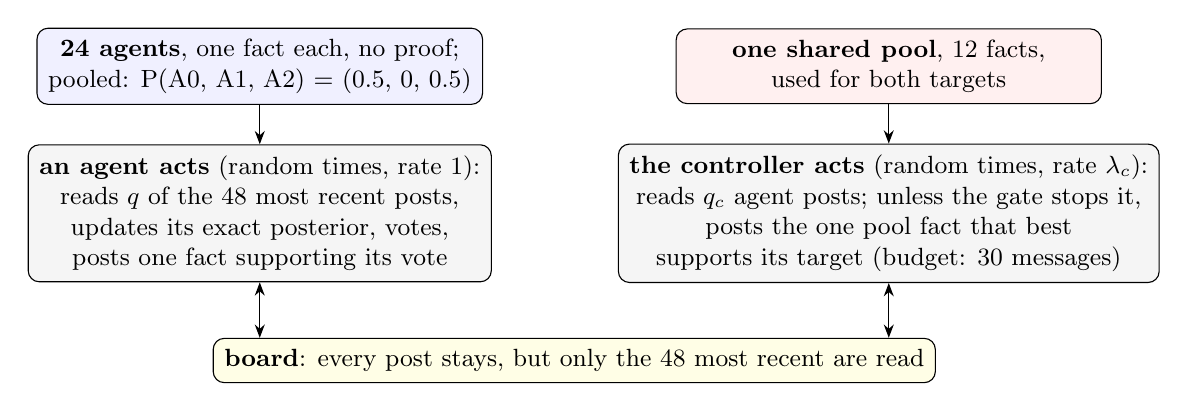
\begin{tikzpicture}[font=\small, box/.style={draw, rounded corners, align=center, inner sep=4pt}]
  \node[box, fill=gray!8, minimum width=5.4cm] (agent) {\textbf{an agent acts} (random times, rate 1):\\
     reads $q$ of the 48 most recent posts,\\ updates its exact posterior, votes,\\ posts one fact supporting its vote};
  \node[box, fill=gray!8, right=1.6cm of agent, minimum width=5.4cm] (ctrl) {\textbf{the controller acts} (random times, rate $\lambda_c$):\\
     reads $q_c$ agent posts; unless the gate stops it,\\ posts the one pool fact that best\\ supports its target (budget: 30 messages)};
  \node[box, fill=blue!6, above=0.5cm of agent, minimum width=5.4cm] (agents) {\textbf{24 agents}, one fact each, no proof;\\
     pooled: P(A0, A1, A2) = (0.5, 0, 0.5)};
  \node[box, fill=red!6, above=0.5cm of ctrl, minimum width=5.4cm] (pool) {\textbf{one shared pool}, 12 facts,\\
     used for both targets};
  \coordinate (mid) at ($(agent.south)!0.5!(ctrl.south)$);
  \node[box, fill=yellow!10, anchor=north, minimum width=8cm] (board) at ($(mid)+(0,-0.7)$) {\textbf{board}: every post stays, but only the 48 most recent are read};
  \draw[-{Stealth}] (agents) -- (agent);
  \draw[-{Stealth}] (pool) -- (ctrl);
  \draw[{Stealth}-{Stealth}] (agent.south) -- (agent.south |- board.north);
  \draw[{Stealth}-{Stealth}] (ctrl.south) -- (ctrl.south |- board.north);
\end{tikzpicture}
\diagramcaption{Simulation 2. There are no rounds. Each remembered fact is forgotten after a
random lifetime (on average a fraction $\rho$ survives one time unit) and comes back if read
again. The controller acts for $0 \le t < 30$; agents continue alone until $t = 40$.}
\end{center}

\noindent The agents' facts plus the \emph{whole} pool give P(A0, A1, A2) = (0.75, 0, 0.25):
the truth keeps an edge that cannot be designed away, because every fact is true. Agents are
exact Bayesian reasoners and vote by probability matching (the vote is drawn from the
posterior). The \emph{vote gate} keeps the controller silent when at least 75\% of the posts
it read come from agents who voted for its target. The grid: posts read $q \in \{3,6,12\}$,
$q_c \in \{3,6,12,24\}$, memory $\rho \in \{0.75, 1\}$, controller rate
$\lambda_c \in \{0.5,1,2,4,8\}$ actions per time unit, gate on/off; 1{,}000 episodes per
setting. Control is measured by the \emph{gain}
\begin{equation}\label{eq:gain}
G(t) = \frac{1}{E}\sum_{e=1}^{E}\Bigl[m_{\text{target}}(t)^{\text{ctrl}}(e) - m_{\text{target}}(t)^{\text{silent}}(e)\Bigr],
\end{equation}
where $m_k(t)$ is the agents' mean belief in allocation $k$ and each episode $e$ uses the same
random draws with and without the controller. (Simulation 1 measures the gain in the share of
\emph{votes}; Figure~\ref{fig:votes} shows the vote shares of both simulations on the same scale.)
Unless stated otherwise: $q = 6$, $q_c = 12$, $\lambda_c = 1$, gate on.

\section{Main result: both controllers tip the swarm, and the effect stays}

\begin{figure}[H]
\centering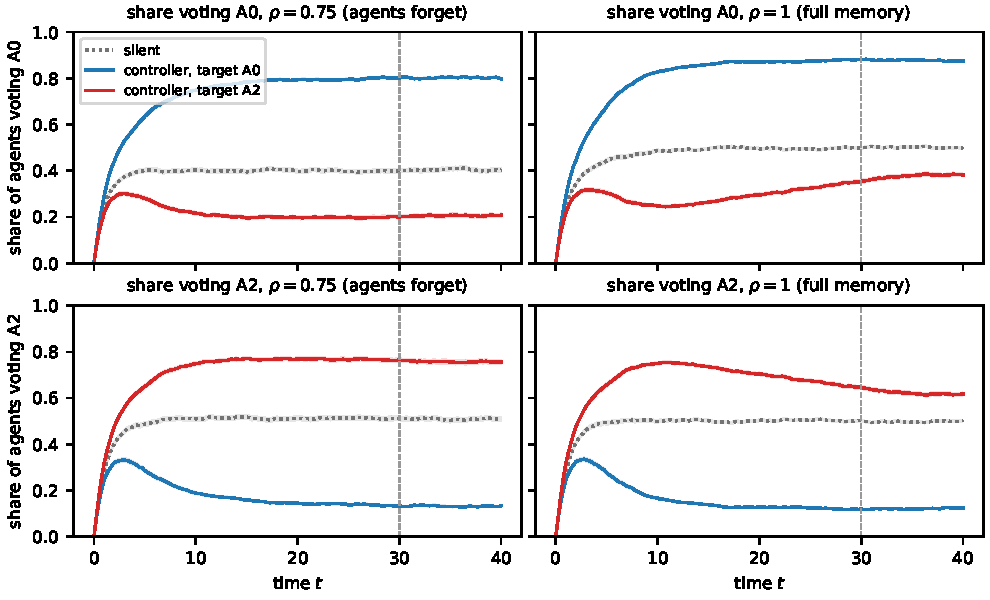
\includegraphics[width=0.84\linewidth]{figures/fig_votes_time.pdf}
\caption{Share of the 24 agents voting A0 (top) and A2 (bottom) over time, without a controller
(dotted grey), with the controller targeting A0 (blue) and with the one targeting A2 (red);
$\rho = 0.75$ (left) and $\rho = 1$ (right). Agents who have not acted yet have no vote, so the
shares start at 0 (all agents have voted by $t \approx 5$). The controller stops at $t = 30$
(dashed). Bands: 95\% intervals. $q = 6$, $q_c = 12$, $\lambda_c = 1$, gate on.}
\label{fig:votes}
\end{figure}

\begin{itemize}\itemsep1pt
\item \textbf{Without a controller the swarm stays split}: at $t = 30$, 40\% vote A0 and 51\% A2
  when agents forget, 50\% each with full memory.
\item \textbf{Either controller tips it within about ten time units}: the target's share reaches
  0.80 (A0) or 0.77 (A2) when agents forget, and 0.88 (A0) or 0.65 (A2) with full memory.
\item \textbf{With full memory the false controller's lead erodes}: the A2 share peaks at 0.76
  ($t \approx 11$) and falls to 0.62 by $t = 40$, as agents accumulate the evidence that favours A0.
\end{itemize}

\begin{table}[H]
\centering\small
\caption{Gain at $t = 30$, $\lambda_c = 1$, gate on: in mean belief, Eq.~(\ref{eq:gain}) (in brackets
the silent swarm's belief in the target), and in the share of votes for the target, the measure of
Simulation 1. Simulation 1: one fact per night, same $q$, $q_c$, $\rho$ (there the two measures agree
within 0.01).}
\label{tab:main}
\begin{tabular}{llcccc}
\toprule
 & & \multicolumn{2}{c}{Simulation 2} & Simulation 1 & \\
$\rho$ & controller & belief & votes & votes & messages sent \\
\midrule
0.75 & truth (A0) & 0.29 (0.38) & 0.40 & 0.42 & 11 \\
0.75 & false (A2) & 0.19 (0.48) & 0.25 & 0.29 & 12 \\
1 & truth (A0) & 0.38 (0.50) & 0.38 & 0.38 & 7 \\
1 & false (A2) & 0.14 (0.50) & 0.14 & 0.15 & 15 \\
\bottomrule
\end{tabular}
\end{table}

\begin{figure}[H]
\centering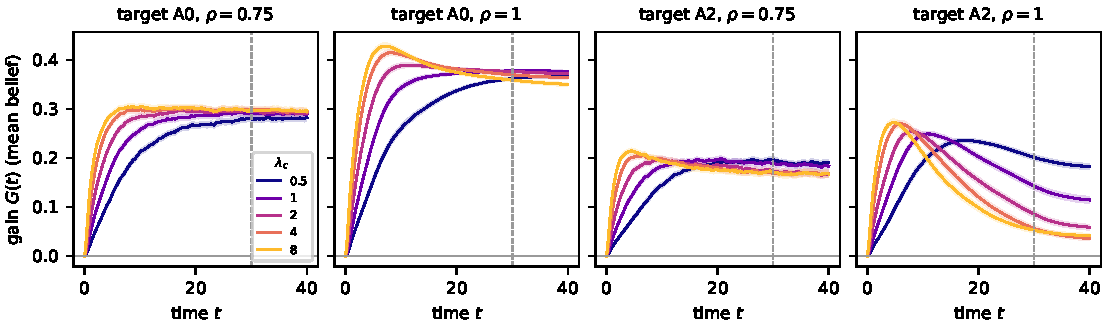
\includegraphics[width=0.98\linewidth]{figures/fig_gain_time.pdf}
\caption{Gain over time, Eq.~(\ref{eq:gain}), one line per controller rate $\lambda_c$; gate on.
The controller stops at $t = 30$ (dashed). Bands: 95\% intervals.}
\label{fig:gaintime}
\end{figure}

\begin{figure}[H]
\centering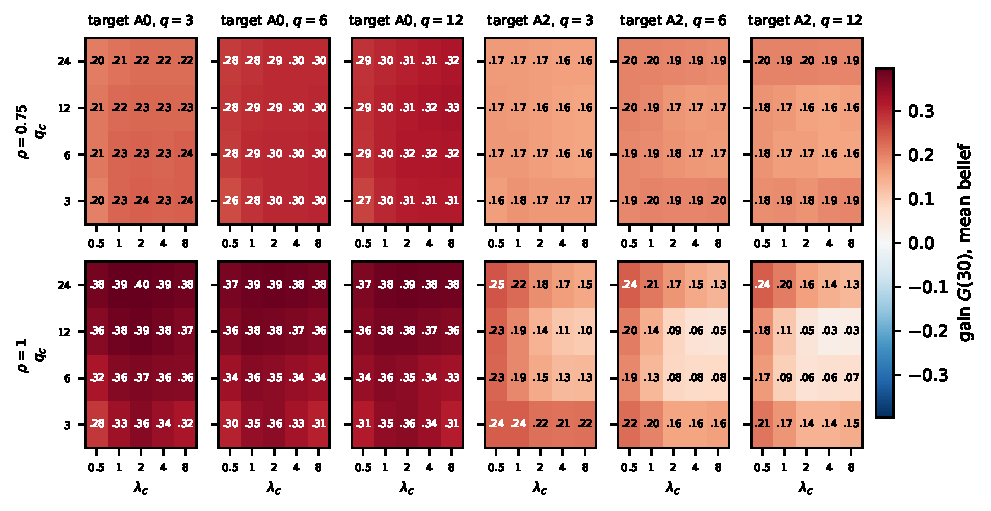
\includegraphics[width=0.98\linewidth]{figures/fig_phase_gain.pdf}
\caption{Gain $G(30)$ over the controller rate $\lambda_c$ (x) and the posts it reads $q_c$ (y), for
each target and every $q$ (columns), $\rho = 0.75$ and $1$ (rows); gate on. Grey number: the 95\%
interval includes 0.}
\label{fig:phase}
\end{figure}

\begin{itemize}\itemsep1pt
\item \textbf{Both controllers tip the swarm} (Table~\ref{tab:main}); the truth controller's
  gain is larger, mostly because the silent swarm already leans to A2 when agents forget
  (Figure~\ref{fig:votes}): there is more room to raise A0.
\item \textbf{In votes, control is about as strong as in Simulation 1}: $0.40$ against $0.42$
  (truth) and $0.25$ against $0.29$ (false) when agents forget; with full memory the two agree
  within $0.01$. \textbf{In mean belief it looks weaker} when agents forget, by $0.13$ (truth) and
  $0.09$ (false), a difference confirmed with fresh random draws. The two measures part because an
  agent votes right after reading, with a fresh memory, and then keeps forgetting until it acts
  again, so a belief snapshot at a fixed time catches agents with faded memories (truth controller,
  $\rho = 0.75$: 80\% vote A0 at $t = 30$, but the mean belief in A0 is 0.67; in Simulation 1 the day-end snapshot comes before
  dawn's forgetting, and beliefs and votes agree). Earlier reports read the belief gap as weaker
  control; the vote gap says the collective decision is affected much less.
\item \textbf{The effect persists}: ten time units after the controller stops, the gain has
  changed by at most $0.016$ at $\rho = 0.75$ (Figure~\ref{fig:gaintime}); agents keep
  relaying the controller's facts (12--45\% of their posts). With full memory a fast false
  controller peaks early and then loses most of its gain (Section~\ref{sec:strength}).
\end{itemize}

\section{The controller's strength and the vote gate}\label{sec:strength}

\subsection{Strength: the controller's rate}

\begin{figure}[H]
\centering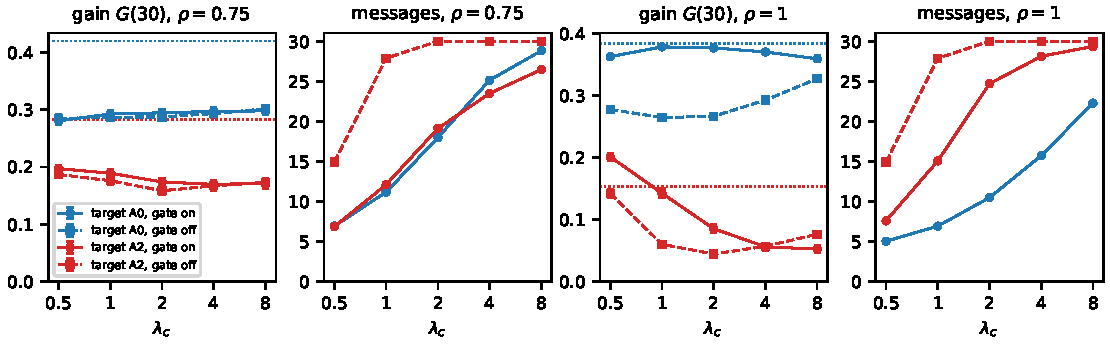
\includegraphics[width=0.98\linewidth]{figures/fig_rate.pdf}
\caption{Gain at $t = 30$ and messages sent against the controller rate, for $\rho = 0.75$
and $\rho = 1$ (target A0 blue, A2 red; gate on solid, off dashed; dotted: Simulation 1).}
\label{fig:rate}
\end{figure}

\paragraph{When agents forget, the rate barely matters.} From $\lambda_c = 0.5$ to $8$ the gain
moves from $0.28$ to $0.30$ (truth) and from $0.20$ to $0.17$ (false), but the messages sent
rise from about 7 to 26--29. A fast controller spends its budget early (by $t \approx 4$ with
the gate off), reaches its gain sooner, and then the gain stays put. Gain per message is
highest for a slow, gated controller.

\paragraph{With full memory, a faster controller steers less.} The false controller's gain
falls from $0.20$ at $\lambda_c = 0.5$ to $0.05$ at $\lambda_c = 8$, and with the gate off the truth controller
loses $0.05$ on average against the gate on, up to $0.12$ (Figure~\ref{fig:rate}, right). The
same fall appears at every $q$ and at $q_c$ = 3, 6 and 12 (Figure~\ref{fig:phase}, bottom row).

\begin{figure}[H]
\centering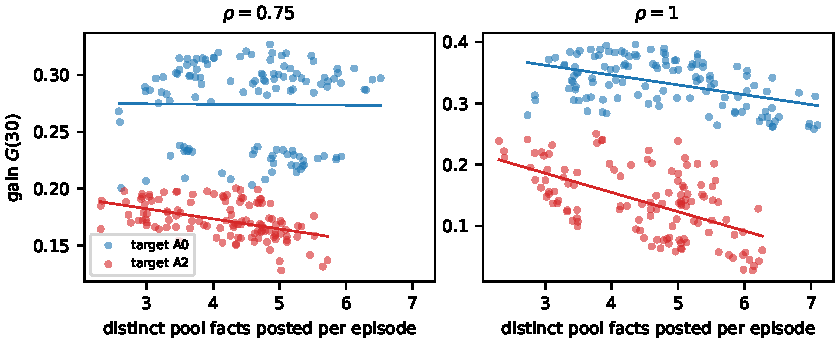
\includegraphics[width=0.66\linewidth]{figures/fig_distinct.pdf}
\caption{Each point is one setting ($q$, $q_c$, $\lambda_c$, gate): gain at $t = 30$ against the
number of different pool facts the controller posted per episode. Lines: least-squares fits.}
\label{fig:distinct}
\end{figure}

\noindent\textbf{Why: saying more of the pool pulls toward the same point.} Every fact is true,
and the agents' facts plus the whole pool give (0.75, 0, 0.25). With full memory nothing posted
is forgotten, so the more \emph{different} pool facts a controller puts into circulation, the
closer beliefs move to that point, whatever its target: down from the false controller's
side, and down from the truth controller's best, which lies above 0.75. At $\rho = 1$ each
additional distinct fact lowers the gain by $0.031$ (false) and $0.016$ (truth)
(Figure~\ref{fig:distinct}, right). The rate sets that number: spread over 30 time units, the
controller reads varied boards and posts more different facts (6.3 per episode at
$\lambda_c = 1$, gate off); at $\lambda_c = 8$ it spends its budget in a burst on similar boards
and repeats itself (5.0), which is why the gain partly recovers there. When agents forget,
facts leave again and the effect is weak (Figure~\ref{fig:distinct}, left). This was found
after looking at the data, so it was rerun with fresh random draws: \textbf{every one of the 16 checked reversals
reappeared} (false controller, gain at $\lambda_c = 0.5 \ldots 8$: 0.20, 0.15, 0.08, 0.05,
0.05). The explanation by distinct facts rests on a correlation across settings and is not yet
tested directly (for example with a controller that remembers what it has said). Simulation 1 has
a different route to the same outcome: there a large posting budget forces facts against the
target onto the board.

\subsection{The vote gate}

The gate keeps the controller silent when it reads enough support. Turning it off adds about
16 messages per episode at $\lambda_c = 1$ (confirmed with fresh draws) and \textbf{no control} when agents
forget ($-0.017$ and $-0.003$); with full memory it \emph{lowers} the gain (truth $-0.05$ on
average) through the mechanism above.

\section{The controller overestimates its support}

\begin{figure}[H]
\centering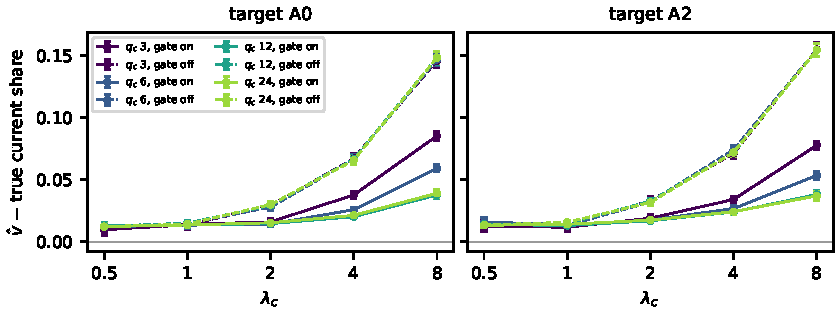
\includegraphics[width=0.66\linewidth]{figures/fig_sensing.pdf}
\caption{Error of the controller's estimate $\hat v$ (share of posts read whose author voted
for the target) against the true current share of all 24 agents' last votes; $\rho = 0.75$;
solid gate on, dashed off.}
\label{fig:sensing}
\end{figure}

Unlike in Simulation 1, $\hat v$ is biased upward, and \textbf{the faster the controller, the
larger the bias}: about $+0.014$ at $\lambda_c \le 1$, rising to $+0.05$ (gate on) and $+0.15$
(gate off) at $\lambda_c = 8$. A likely reason, not yet tested: the posts it reads come from agents who
acted recently, often just after reading the controller's facts, while the true share also
counts older votes. More posts read ($q_c$) reduce the error's spread (0.16 at $q_c = 3$, 0.07
at $q_c = 24$) but not the bias.

%% ---------------------------------------------------------------------------------------------
\section{How readable is the command? Information and pair efficiency}\label{sec:eff}

A controller can change the swarm in two ways: in the direction it is asked to, or in ways that
happen whatever its target. We measure how readable the command is in the swarm (the mutual
information between the target and the swarm's state), which share of the change is directed (the
pair efficiency $\eta$), and how unsure the agents become. Throughout, the target is chosen by a fair
coin, and all quantities are taken at one time $t$, across the 1{,}000 episodes of each arm (not over
whole trajectories). Setting: $q = 6$.

\subsection{Measures}

\begin{center}
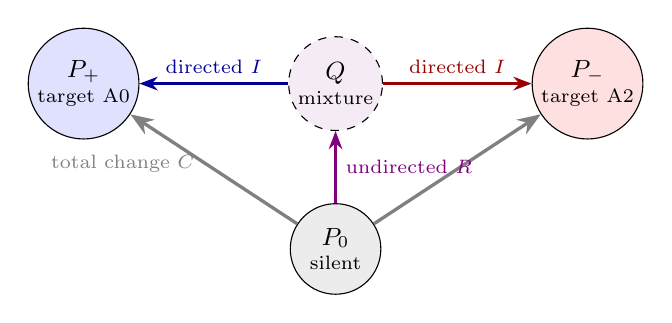
\begin{tikzpicture}[font=\small, dist/.style={draw, circle, minimum size=1.15cm, align=center, inner sep=1pt}]
  \node[dist, fill=gray!15] (P0) at (0,0) {$P_0$\\[-2pt]{\scriptsize silent}};
  \node[dist, fill=blue!12] (Pp) at (-3.2,2.1) {$P_+$\\[-2pt]{\scriptsize target A0}};
  \node[dist, fill=red!12] (Pm) at (3.2,2.1) {$P_-$\\[-2pt]{\scriptsize target A2}};
  \node[dist, dashed, fill=violet!8] (Q) at (0,2.1) {$Q$\\[-2pt]{\scriptsize mixture}};
  \draw[-{Stealth}, very thick, gray] (P0) -- node[left, font=\scriptsize, pos=0.55]{total change $C$} (Pp);
  \draw[-{Stealth}, very thick, gray] (P0) -- (Pm);
  \draw[-{Stealth}, thick, violet] (P0) -- node[right, font=\scriptsize]{undirected $R$} (Q);
  \draw[-{Stealth}, thick, blue!60!black] (Q) -- node[above, font=\scriptsize]{directed $I$} (Pp);
  \draw[-{Stealth}, thick, red!60!black] (Q) -- node[above, font=\scriptsize]{directed $I$} (Pm);
\end{tikzpicture}
\diagramcaption{Three distributions of the swarm's state at time $t$, one per arm, each over the
episodes of that arm. The controller's total change $C$ splits exactly into a part that depends on
its target ($I$, from the mixture $Q$ to each arm) and a part that does not ($R$, from silence to
$Q$). Efficiency $\eta = I/C$ is the directed share.}
\end{center}

\noindent\textbf{Distributions.} For each arm $a$ (silent $0$, target A0 $+$, target A2 $-$) and a
time $t$, each episode $e$ contributes a probability vector $y_a(e)$ over the values $x$ of the
state $X$: at \emph{one-agent} level its vote shares (the vote of a randomly chosen agent), at
\emph{swarm} level a mark on the bin of $s = m_{\text{A0}} - m_{\text{A2}}$ (difference of mean
beliefs, three equal bins on $[-1,1]$). Then $\hat P_a = \frac1n\sum_e y_a(e)$. Any pair of controllers
can be written as
\begin{equation}\label{eq:split}
\hat P_\pm = \hat P_0 + \mu \pm \delta,\qquad \mu = \tfrac12(\hat P_+ + \hat P_-) - \hat P_0,\quad
\delta = \tfrac12(\hat P_+ - \hat P_-),
\end{equation}
a \emph{common} part $\mu$ (what control does on average, whatever the target) and a
\emph{directional} part $\delta$; both are vectors over the values of $X$ (all answers, A1 included).

\noindent\textbf{Readability and the pair efficiency.} With $\hat Q = \hat P_0 + \mu$ and
$\mathrm{KL}(p\Vert q) = \sum_x p(x)\log_2[p(x)/q(x)]$,
\begin{equation}\label{eq:eta}
I = \tfrac12\mathrm{KL}(\hat P_+\Vert\hat Q) + \tfrac12\mathrm{KL}(\hat P_-\Vert\hat Q),\quad
C = \tfrac12\mathrm{KL}(\hat P_+\Vert\hat P_0) + \tfrac12\mathrm{KL}(\hat P_-\Vert\hat P_0) = I + R,\quad
R = \mathrm{KL}(\hat Q\Vert\hat P_0),\quad \eta = I/C .
\end{equation}
$I$ is the mutual information between the target and the state: how readable the command is
(at most 1 bit). With the one-agent state it is $I(\text{target};\text{vote of a randomly chosen
agent})$, the quantity mapped in Figure~\ref{fig:effI}. $I = \frac12\mathrm{KL}(\hat Q+\delta\Vert\hat Q) + \frac12\mathrm{KL}(\hat Q-\delta\Vert\hat Q)$
depends on $\delta$ and on where the pair sits ($\hat Q$); $R = \mathrm{KL}(\hat P_0+\mu\Vert\hat P_0)$ depends
only on $\mu$; $C$ (a number) $= I + R$, so $R = C - I$. The reference $\hat P_0$ is the silent arm. For
small changes, $\mathrm{KL}(p+\epsilon\Vert p) \approx \sum_x \epsilon(x)^2/(2\ln 2\,p(x))$ gives
\begin{equation}\label{eq:etasmall}
I \approx \frac{\Vert\delta\Vert^2}{2\ln 2},\quad R \approx \frac{\Vert\mu\Vert^2}{2\ln 2},\quad
\eta \approx \frac{1}{1 + \Vert \mu\Vert^2/\Vert\delta\Vert^2},\qquad \Vert v\Vert^2 = \sum_x \frac{v(x)^2}{\hat P_0(x)} .
\end{equation}
So $\eta = 1$ exactly when the two controllers' changes are mirror images ($\mu = 0$), whatever their
size, and $\eta$ falls only through the \emph{ratio} of common to directional change: when both push
the same way (a common push), or one moves the swarm much more than the other (a lopsided pair:
along one direction with sizes $a$ and $b$, $\Vert \mu\Vert/\Vert\delta\Vert = |a-b|/(a+b)$). It is a
property of the pair, not of either controller, and it stays constant whenever both effects grow
together; the size of the effect is measured by $I$. At swarm level $C$ is often infinite (the
controlled swarm reaches states silence never visits); there we use $\eta_{JS} = I/(I + \mathrm{JS}(\hat Q,\hat P_0))$ with the bounded
Jensen--Shannon divergence; $\mathrm{JS}(\hat Q,\hat P_0)$ is the information the state carries about
\emph{whether} a controller is present (controlled or silent, 50/50), so $\eta_{JS}$ compares
information about the direction with information about the presence of control.

\noindent\textbf{The agents' own uncertainty}: $\Delta\bar H$ (change in the mean entropy of their
beliefs) and $\Delta$JSD (change in disagreement, the entropy of the mean belief minus $\bar H$),
controlled minus silent, same episode.

\subsection{Over time}

\begin{figure}[!htb]
\centering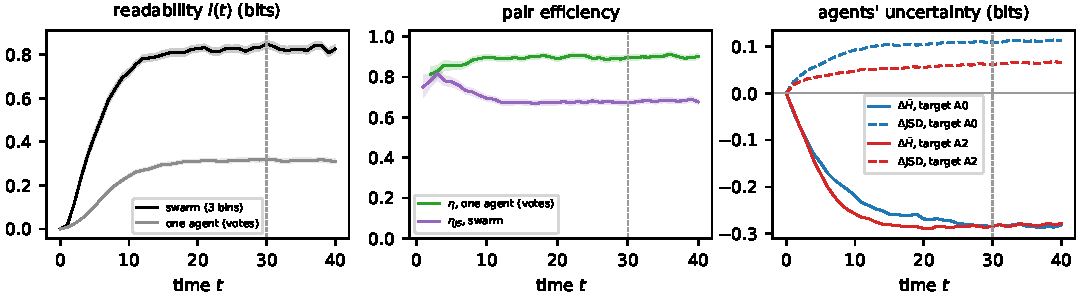
\includegraphics[width=0.92\linewidth]{figures/fig_eff_time2.pdf}
\caption{At $\rho = 0.75$, $q_c = 12$, $\lambda_c = 1$, gate on (the controller stops at $t = 30$,
dashed): readability $I(t)$ at swarm and one-agent level, pair efficiency ($\eta$, one agent;
$\eta_{JS}$, swarm), and the change in the agents' uncertainty. Bands: 95\% intervals over episodes.}
\label{fig:efftime2}
\end{figure}

\begin{figure}[!htb]
\centering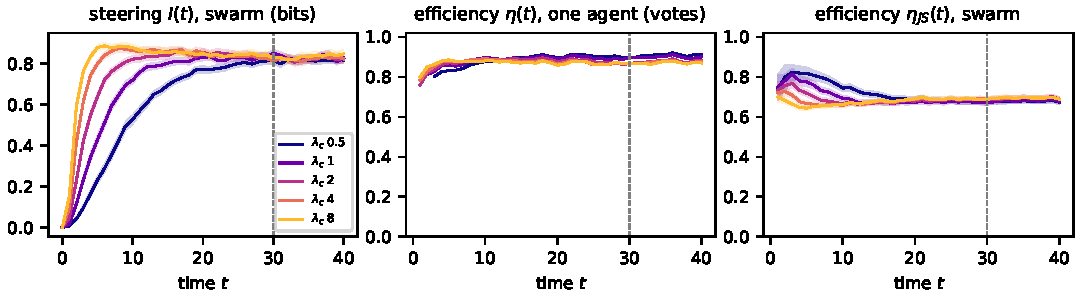
\includegraphics[width=0.66\linewidth]{figures/fig_eff_time.pdf}
\caption{Readability and pair efficiency over time, $\rho = 0.75$, $q_c = 12$, gate on, one line per
rate; the controller stops at $t = 30$ (dashed). Bands: 95\% intervals.}
\label{fig:efftime}
\end{figure}

\begin{itemize}\itemsep1pt
\item \textbf{Readability builds within 10--15 time units and persists}: at $t = 30$, $I = 0.85$ bits
  (swarm) and $0.32$ bits (one agent's vote), almost unchanged at $t = 40$; $\eta = 0.90$,
  $\eta_{JS} = 0.67$. Faster controllers get there sooner; all rates end at the same level.
\item \textbf{Agents become surer} ($\Delta\bar H = -0.28$ bits) \textbf{but disagree more}
  ($\Delta$JSD $+0.11$ for target A0, $+0.06$ for target A2).
\end{itemize}

\subsection{Across the control plane}

\begin{figure}[!htb]
\centering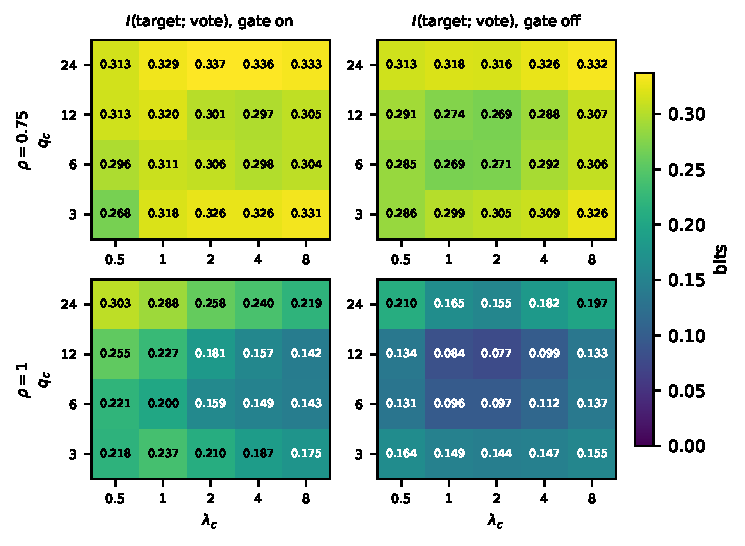
\includegraphics[width=0.6\linewidth]{figures/fig_eff_phase_I.pdf}
\caption{Readability $I(\text{target};\text{vote})$ at $t = 30$, in bits, over the reading budget $q_c$ (y)
and the controller rate $\lambda_c$ (x); state: the vote of a randomly chosen agent.}
\label{fig:effI}
\end{figure}

\begin{figure}[!htb]
\centering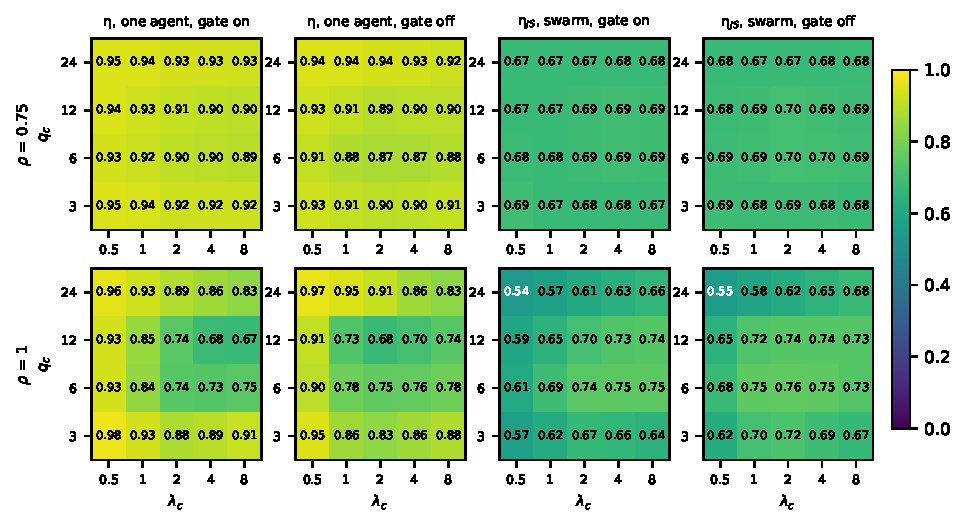
\includegraphics[width=0.62\linewidth]{figures/fig_eff_phase.pdf}
\caption{Pair efficiency at $t = 30$ over $q_c$ and the controller rate $\lambda_c$: one-agent $\eta$ (beliefs) and swarm
$\eta_{JS}$. Dash: undefined.}
\label{fig:effphase}
\end{figure}

\begin{itemize}\itemsep1pt
\item \textbf{When agents forget, readability hardly depends on the settings}: 0.27--0.34 bits for
  every $q_c$, rate and gate (Figure~\ref{fig:effI}, top), and $\eta$ is flat (0.86--0.95).
\item \textbf{With full memory readability falls with the rate}: from 0.30 bits ($q_c = 24$,
  $\lambda_c = 0.5$) to 0.14--0.22 at $\lambda_c = 8$ with the gate on, and lower still with the gate
  off (0.08--0.21). This is the false controller's stall (Section~\ref{sec:strength}): its target
  becomes harder to tell from the truth controller's.
\end{itemize}

\subsection{Readability, pair efficiency and uncertainty against the controller rate}

\begin{figure}[!htb]
\centering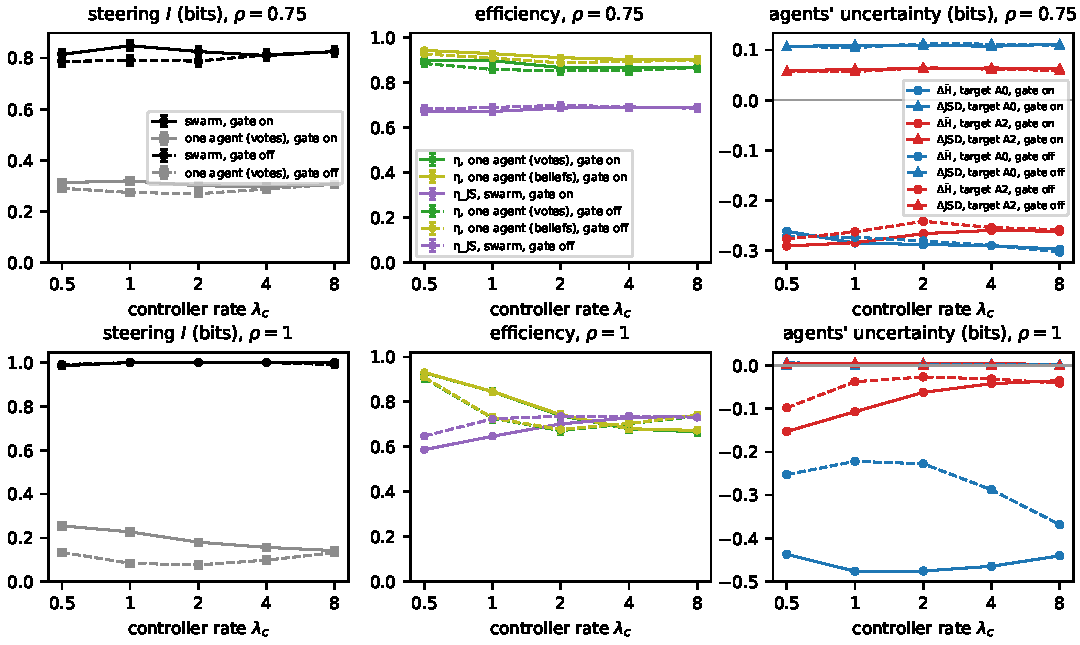
\includegraphics[width=0.72\linewidth]{figures/fig_eff_settings.pdf}
\caption{Readability $I$ (left), pair efficiency (middle) and the change in the agents' uncertainty
(right; circles $\Delta\bar H$, triangles $\Delta$JSD) at $t = 30$ against the controller rate $\lambda_c$ ($q_c = 12$; solid: gate on; dashed: gate off). Bars: 95\% intervals.}
\label{fig:effsettings}
\end{figure}

\begin{itemize}\itemsep1pt
\item \textbf{When agents forget, $\eta$ is flat (0.86--0.95)}: the two controllers' effects grow together.
\item \textbf{With full memory $\eta$ falls with the rate} (0.93 to 0.67) because the pair turns
  lopsided: the false controller's gain collapses, the truth controller's does not. Swarm
  $\eta_{JS}$ moves the other way, because swarm readability is saturated at 1 bit; the one-agent
  measures are the informative ones here.
\end{itemize}

\subsection{Precision at 50, 100 and 300 paths}

\begin{table}[H]
\centering\small
\caption{Value from 1{,}000 paths per arm, and root-mean-square error of the estimate from 50, 100
or 300 paths (200 random subsets each), at $t = 30$, $\lambda_c = 1$, $q_c = 12$, gate on, $\rho = 0.75$.}
\label{tab:effprec}
\begin{tabular}{lcccc}
\toprule
quantity & 1{,}000 paths & error, 50 & error, 100 & error, 300 \\
\midrule
steering $I$, swarm (3 bins) & 0.849 & 0.039 & 0.026 & 0.013 \\
steering $I$, one agent (votes) & 0.320 & 0.023 & 0.017 & 0.009 \\
efficiency $\eta$, one agent (votes) & 0.898 & 0.032 & 0.022 & 0.010 \\
efficiency $\eta_{JS}$, swarm & 0.672 & 0.027 & 0.019 & 0.010 \\
$\Delta\bar H$, target A0 & -0.284 & 0.024 & 0.016 & 0.009 \\
$\Delta\bar H$, target A2 & -0.284 & 0.023 & 0.016 & 0.008 \\
$\Delta$JSD, target A0 & 0.110 & 0.008 & 0.006 & 0.003 \\
$\Delta$JSD, target A2 & 0.062 & 0.008 & 0.006 & 0.003 \\
\bottomrule
\end{tabular}
\end{table}

\noindent Across all settings, at 100 paths: readability $\pm0.01$ (one agent) to $\pm0.03$ (swarm),
$\eta$ $\pm0.02$--$0.03$, $\Delta\bar H$ $\pm0.02$, $\Delta$JSD $\pm0.006$. Two settings that differ by
at least 0.02 are ordered correctly in 90--100\% of subsets.

%% ---------------------------------------------------------------------------------------------
\section{Success against facts posted}\label{sec:success}

The information measures above say how readable the command is, not whether the swarm ends up
deciding what the controller wants, nor at what cost. Here we measure both directly.

\begin{itemize}\itemsep1pt
\item \textbf{Collective decision} $Y_T$: plurality of the agents' last votes at time $T$; a tie
  between $k$ answers counts $1/k$. \textbf{Success}: $Y_T$ = the controller's target.
\item \textbf{Benefit} $\Delta_\pi = p_\pi - p_0$: change in the probability that the target wins,
  against the silent arm of the same episodes; $p_0$ is the silent probability.
\item \textbf{Cost} $C_\pi$: facts actually posted up to $T$, mean per run (not the allowed budget).
\item \textbf{Best-achievable curve} among the tested settings $\pi$ of one group ($\rho$, target):
  $\Delta^*(B) = \max\{\Delta_\pi : C_\pi \le B\}$, the largest gain reached spending at most $B$;
  read the other way, $C^*(\delta) = \min\{C_\pi : \Delta_\pi \ge \delta\}$, the least spending that
  reaches $\delta$. A setting below the curve is \emph{dominated}: another reached at least as much for less.
\item \textbf{Cost efficiency} $\eta_{\text{cost}} = C^*(\Delta_\pi)/C_\pi$: the share of the spending that
  was necessary (1: nothing cheaper reached as much). Not defined where $\Delta_\pi \le 0$ or its
  95\% interval includes 0.
\end{itemize}

\paragraph{How to read the curves.} Each dot is one setting, at (facts posted, gain). The
\textbf{solid line} is the best-achievable curve over the tested settings: it starts at $(0,0)$ (no
control) and steps up each time a setting reaches a higher gain than anything cheaper; dots on it have
$\eta_{\text{cost}} = 1$, dots below it are dominated, and $\eta_{\text{cost}}$ is how far to the left the
curve reaches the same gain. The \textbf{dashed line} is what becomes reachable if the controller
\emph{chooses its setting at random for each run}: using setting X (7 facts, $+0.32$) in half of the
runs and no control in the other half costs 3.5 facts and gains $+0.16$ \emph{on average}, so every
point on the straight segment between two settings (or between a setting and $(0,0)$) is reachable on
average; the dashed line is the outermost such segments (the concave hull through $(0,0)$). It lies above
the solid line where mixing beats every single setting. Its first segment from $(0,0)$ is arithmetic,
not an observation.

\begin{center}
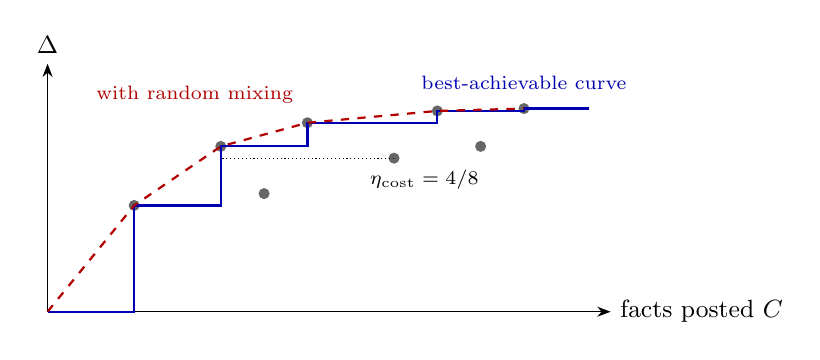
\begin{tikzpicture}[font=\small, x=0.55cm, y=3cm]
  \draw[-{Stealth}] (0,0) -- (13,0) node[right]{facts posted $C$};
  \draw[-{Stealth}] (0,0) -- (0,1.05) node[above]{$\Delta$};
  \foreach \c/\d in {2/0.45, 4/0.7, 6/0.8, 9/0.85, 11/0.86, 5/0.5, 8/0.65, 10/0.7}
     \fill[black!60] (\c,\d) circle (2pt);
  \draw[thick, blue!70!black] (0,0) -- (2,0) -- (2,0.45) -- (4,0.45) -- (4,0.7) -- (6,0.7) -- (6,0.8) -- (9,0.8) -- (9,0.85) -- (11,0.85) -- (11,0.86) -- (12.5,0.86);
  \draw[thick, dashed, red!70!black] (0,0) -- (2,0.45) -- (4,0.7) -- (6,0.8) -- (9,0.85) -- (11,0.86);
  \draw[densely dotted] (8,0.65) -- (4,0.65);
  \node[font=\scriptsize, align=left] at (8.7,0.56) {$\eta_{\text{cost}} = 4/8$};
  \node[font=\scriptsize, blue!70!black] at (11,0.97) {best-achievable curve};
  \node[font=\scriptsize, red!70!black] at (3.4,0.92) {with random mixing};
\end{tikzpicture}
\diagramcaption{Illustration. Each point is a setting. Solid: best-achievable curve; dashed: reachable
on average by random mixing per run. The setting at cost 8 reaches $\Delta = 0.65$, which a setting
costing 4 already reaches: $\eta_{\text{cost}} = 0.5$.}
\end{center}

\begin{figure}[H]
\centering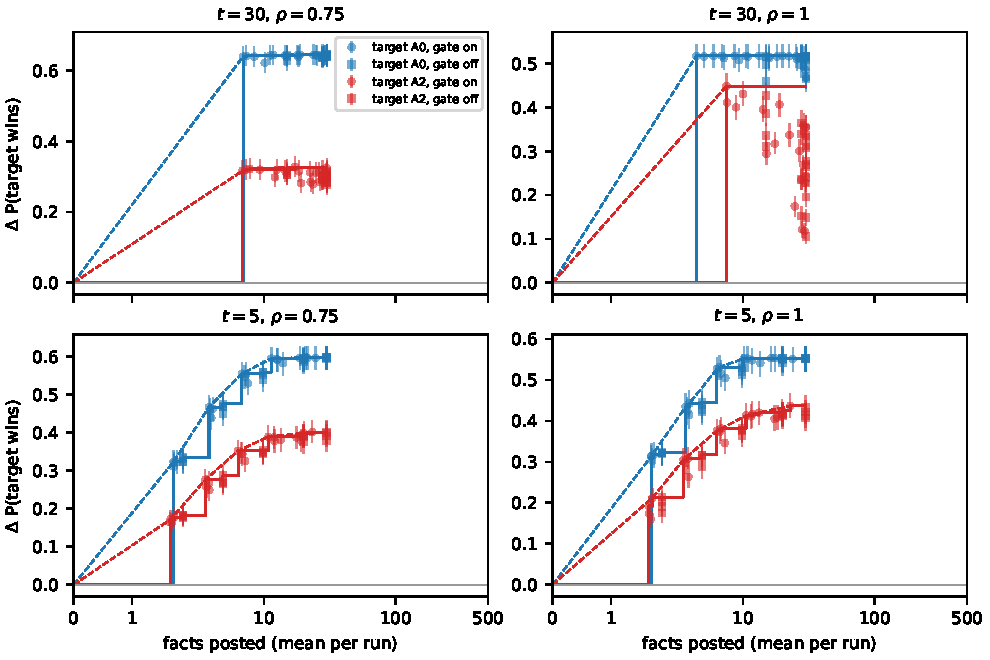
\includegraphics[width=0.84\linewidth]{figures/fig_success_facts.pdf}
\caption{Change in the probability that the controller's target wins against facts posted, at
$t = 30$ (top) and $t = 5$ (bottom), $\rho = 0.75$ (left) and $1$ (right); every setting
($q_c \times \lambda_c \times$ gate, $q = 6$) with its 95\% interval; blue: target A0, red: target A2;
circles gate on, squares gate off. Solid: best-achievable curve; dashed: with random mixing per run.
The x axis is linear from 0 to 1 and logarithmic above, up to 500 as in Simulation 1.}
\label{fig:success}
\end{figure}

\begin{itemize}\itemsep1pt
\item \textbf{At $t = 30$ success saturates with very little control.} When agents forget, every
  setting reaches about the same gain ($+0.62$ to $+0.65$ for target A0, $+0.28$ to $+0.33$ for target
  A2), whatever it spent (7 to 30 facts). The cheapest setting ($\lambda_c = 0.5$, gate on,
  $q_c = 12$; 6.9 facts) is already on the flat part of the curve; the median setting spends two to
  four times more for the same result (median $\eta_{\text{cost}}$ 0.48 for target A0, 0.26 for A2;
  lowest 0.23, gate off at high rates). Spending after the decision is settled buys nothing.
\item \textbf{With full memory only one setting is efficient} for each target ($q_c = 24$,
  $\lambda_c = 0.5$, gate on: 4.4 facts for $+0.52$, target A0; 7.5 facts for $+0.45$, target A2). For
  target A2 more spending is worse: the gain falls to $+0.11$ at 30 facts (the rate reversal of
  Section~\ref{sec:strength}).
\item \textbf{Early on, speed buys success, with diminishing returns.} At $t = 5$ the gain rises with
  the facts posted: target A2 from $+0.16$ (1.9 facts) to $+0.40$ (23 facts), target A0 from $+0.32$ to
  $+0.60$; the first few facts buy most of it, and 14--16 of the 40 settings lie on the curve. By
  $t = 10$ the slow controllers have caught up, so efficiency depends on when success is scored.
\item \textbf{Target A0 gains more than A2 mostly because of where the silent swarm starts}: without
  control A2 wins 64\% of runs and A0 35\% when agents forget (Figure~\ref{fig:votes}). As a share of
  the room left, $\Delta/(1-p_0)$, the two targets are closer (median 0.99 for A0, 0.84 for A2).
\item \textbf{Precision at 100 paths}: $\Delta$ $\pm0.017$; $\eta_{\text{cost}}$ $\pm0.02$--$0.035$. Where gains
  are flat, which setting is ``on the curve'' is decided by differences smaller than this, so single
  values of $\eta_{\text{cost}}$ near 1 among equal gains should not be over-read.
\end{itemize}

\paragraph{Caveats.} One world (task\_003), 24 agents, exact-Bayesian agents,
probability-matching votes; a controller without memory that posts one fact at a time; a
budget of 30 messages. Means over 1{,}000 episodes per setting. Efficiencies are relative to the
tested settings: nothing was tested below about 2 facts ($t = 5$) or 7 facts ($t = 30$). Full
analysis, code and tables: \texttt{analysis/task003\_llm\_free/simulation\_2/analysis/} (report of
9 October, reviewer guide) and \texttt{analysis/task003\_llm\_free/efficiency\_estimates/}.

\end{document}
